\chapter{Perception of Rhetorical Tactics in Individual Comments}
\label{perception}

This chapter examines how
\TODO{intro}


\section{Methodology}

\subsection{Data Sample}
\label{perception1:method:sample}
Social media posts for this experiment were sourced from Facebook, Twitter and Reddit (specifically, in this instance, the World News ``subreddit''\footnote{https://www.reddit.com/r/worldnews/}).

From Facebook and Twitter, posts were collected by gathering the 100 most recent posts from five major news distribution networks (\textit{BBC News}, \textit{Sky News}, \textit{CNN News}, \textit{The Guardian}, and \textit{The Daily Mail}) and all replies associated with them. Because these institutions do not main a high-profile, active presence on Reddit, this potion of the data sample was sourced instead by collecting the top 500 ``hot'' posts.

These threads were then pruned to ensure they contained some form of discourse; that is to say they contained at least two replies, made by at least two different users. Applying this filter resulted in 500 threads from Facebook, 403 from Twitter and 247 from Reddit.

These threads were then examined based on a number of different factors to determine the shape of a ``typical'' thread for each platform.
These factors were the \textit{total comments}, \textit{comment length}, \textit{comments per user} and \textit{replies}. \CITATION
Tables \ref{table:perception:number_comment}, \ref{table:perception:comment_length}, \ref{table:perception:comments_per_user}, and \ref{table:perception:replies} show a further breakdown of each of the measures used to determine a typical thread for this purpose. These graphs are also shown in Appendix \ref{socialgraphs}.

Table \ref{table:perception:number_comment} (and Graphs \ref{socialgraphs:comments:facebook}, \ref{socialgraphs:comments:twitter} and \ref{socialgraphs:comments:reddit}) shows the distribution of the total number of comments in each thread. \TODO{Of interest is}

Table \ref{table:perception:comment_length} \TODO{and Graph X.X?} shows the distribution of the average comment length in each thread. \TODO{Of interest is}

Table \ref{table:perception:comments_per_user} \TODO{and Graph X.X?} shows the distribution of the total number of comments made by each user, in each thread. \TODO{Of interest is}

Table \ref{table:perception:replies} \TODO{and Graph X.X?} shows the distribution of the total number of direct replies to other comments within each thread. \TODO{Of interest is}

Threads that fell outside of the interquartile range were removed from the sample. This left 139 Facebook threads (with a total of 14,556 individual posts), 113 Twitter threads (with a total of 1,021 individual posts), and 52 Reddit threads (with a total of 1,123 individual posts.



\begin{table}
\centering
\caption{\TODO{Double check some of these numbers;} Summary of median attributes of platform threads}
\label{table:perception:median_summary}
\begin{tabular}{ l | p{3cm} | p{3cm} | p{3cm} | p{3cm}}
\textbf{Platform} & \textbf{Median number of comments} & \textbf{Median length of comments} & \textbf{Median comments per user} & \textbf{Median internal replies} \\
\hline
Facebook & 95.0 & 103.0 & 1.0 & 0.0\\
\hline
Twitter & 7.5 & 87.0 & 1.0 & 6.0\\
\hline
Reddit & 5.0 & 173.0 & 1.0 & 2.0\\
\end{tabular}
\end{table}

\begin{table}
\centering
\caption{Distribution of number of comments in each thread}
\label{table:perception:number_comment}
\begin{tabular}{ l | l | l | l | l | l | l | l}
\textbf{Platform} & \textbf{Minimum} & \textbf{Lower Quartile} & \textbf{Median} & \textbf{Upper Quartile} & \textbf{Maximum} & \textbf{Mean} & \textbf{$\sigma$}\\
\hline
Facebook & 3.0 & 39.0 & 95.0 & 215.5 & 3958.0 &  & \\
\hline
Twitter & 1.0 & 4.0 & 7.5 & 15.0 & 95.0 &  & \\
\hline
Reddit & 1.0 & 2.0 & 5.0 & 21.0 & 2490.0 &  & \\
\end{tabular}
\end{table}

\begin{table}
\centering
\caption{Distribution of comment length (in characters) in each thread}
\label{table:perception:comment_length}
\begin{tabular}{ l | l | l | l | l | l | l | l}
\textbf{Platform} & \textbf{Minimum} & \textbf{Lower Quartile} & \textbf{Median} & \textbf{Upper Quartile} & \textbf{Maximum} & \textbf{Mean} & \textbf{$\sigma$}\\
\hline
Facebook & 24.0 & 68.0 & 103.0 & 151.5 & 970.0 &  & \\
\hline
Twitter & 34.0 & 73.0 & 87.0 & 99.0 & 140.0 &  & \\
\hline
Reddit &  7.0 & 95.0 & 173.0 & 276.0 & 9874.0 &  & \\
\end{tabular}
\end{table}

\begin{table}
\centering
\caption{Distribution of the number of comments per user in each thread}
\label{table:perception:comments_per_user}
\begin{tabular}{ l | l | l | l | l | l | l | l}
\textbf{Platform} & \textbf{Minimum} & \textbf{Lower Quartile} & \textbf{Median} & \textbf{Upper Quartile} & \textbf{Maximum} & \textbf{Mean} & \textbf{$\sigma$}\\
\hline
Facebook & 1.0 & 1.0 & 1.0 & 1.0 & 1.0 &  & \\
\hline
Twitter & 1.0 & 1.0 & 1.0 & 1.0 & 4.0 &  & \\
\hline
Reddit & 1.0 & 1.0 & 1.0 & 1.0 & 4.0 &  & \\
\end{tabular}
\end{table}

\begin{table}
\centering
\caption{Distribution of the number of internal replies in each thread}
\label{table:perception:replies}
\begin{tabular}{ l | l | l | l | l | l | l | l}
\textbf{Platform} & \textbf{Minimum} & \textbf{Lower Quartile} & \textbf{Median} & \textbf{Upper Quartile} & \textbf{Maximum} & \textbf{Mean} & \textbf{$\sigma$}\\
\hline
Facebook & 0.0 & 0.0 & 0.0 & 0.0 & 0.0 &  & \\
\hline
Twitter & 0.0 & 3.0 & 6.0 & 13.0 & 92.0 &  & \\
\hline
Reddit & 0.0 & 0.0 & 2.0 & 15.0 & 1998.0 &  & \\
\end{tabular}
\end{table}


Each of these ``normal'' threads was then annotated by topic, using one of the following categories based on an aggregation of the topics provided by the five news distribution sites the social media accounts of which the stories were sourced from:
\textit{Current Events}, stories covering recent or ongoing occurrences;
\textit{Business}, stories involving businesses and/or the economy;
\textit{Politics}, stories relating to politics, politicians, elections, etc.;
\textit{Science \& Technology}, stories relating to science, the environment, new technologies, etc.;
\textit{Entertainment \& Arts}, stories involving cultural events, celebrities, etc.;
\textit{Sports}, stories covering sporting events and participants;
and \textit{Features}, stories that form an opinion piece, or focus on an individual rather than the broader story they are a part of.


\begin{table}
\centering
\caption{Threads by topic}
\label{table:perception:replies}
\begin{tabular}{ l | l | l | l | l}
\textbf{Platform} & \textbf{Current Events} & \textbf{Business} & \textbf{Politics} & \textbf{Science \& Technology} \\
\hline
Facebook & 52 & 18 & 23 & 16 \\
\hline
Twitter & 53 & 3 & 24 & 12\\
\hline
Reddit & 41 & 4 & 2 & 6\\
\end{tabular}
\newline
\newline
\begin{tabular}{ l | l | l | l}
\textbf{Platform} & \textbf{Entertainment \& Arts} & \textbf{Sports} & \textbf{Feature}\\
\hline
Facebook & 20 & 3 & 32 \\
\hline
Twitter & 12 & 3 & 20 \\
\hline
Reddit & 2 & 0 & 0 \\
\end{tabular}
\end{table}
 

\subsection{Classifications}

\TODO{Argument}

\TODO{Social} 
 \citet{kietzmann2011social} describe seven
Identity, Sharing, Presence, Relationships, Reputation, Groups, and Conversations



Table \ref{table:perception:questions} summarises each of these classifications, and provides justification for their inclusion.

\subsection{Participants and Survey}
Participants were invited via a general call on social media; they were provided an information sheet and consent form, and asked to confirm that they were above the age of eighteen. 
Participants were shown a post taken from the sample described in Section \ref{perception1:method:sample};
These were presented to participants via a web-survey, a screenshot of which is shown in Figure \ref{figure:perception:survey}.

\begin{figure}
\centering
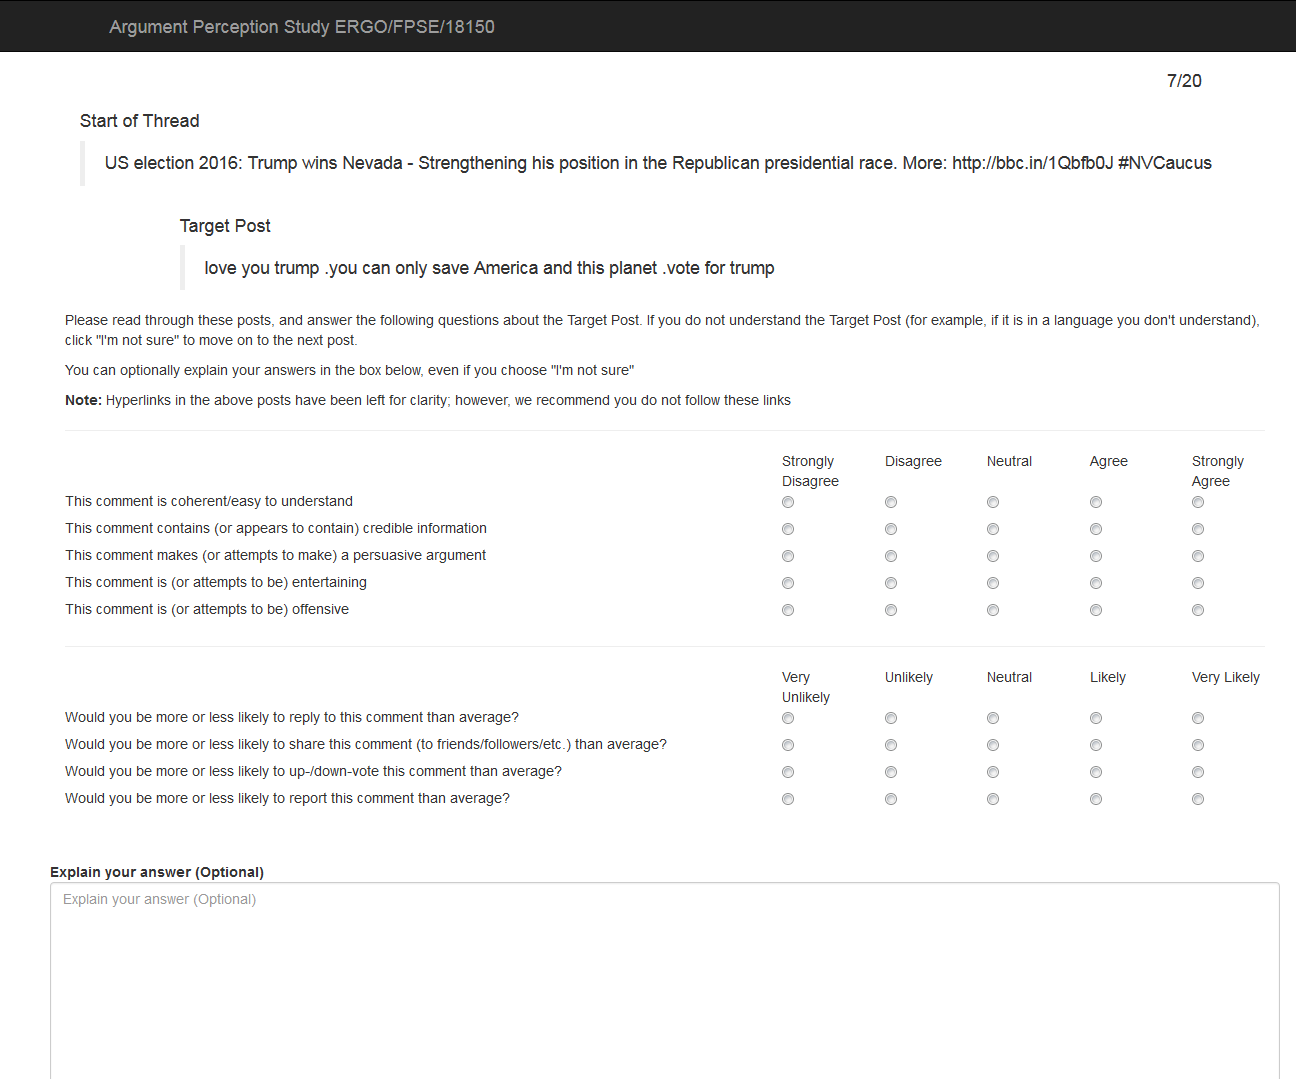
\includegraphics[scale=0.45]{perception/survey1.png}
\caption{The questionnaire as presented to participants}
\label{figure:perception:survey}
\end{figure}


Every participant was also shown, and asked to rate, two additional posts common to all participants to judge the overall inter-rater agreement. These were selected at random from the sampled pool of comments and manually inspected to ensure they were non-empty and comprehensible (e.g., English-language).


\begin{table}
\centering
\caption{Example classifications of argumentation posts}
\label{table:perception:questions}
\begin{tabular}{ l | p{10cm}}
\textbf{Factor} & \textbf{Description} \\
\hline
Coherence & How clear and understandable the post is \CITATION  \\
\hline
Credibility & Whether the post contains (purportedly) credible information \CITATION \\
\hline
Persuasiveness & \citep{sundar2000}\\
\hline
Entertainment & \citep{sundar2000}\\
\hline
Offence & \\
\hline
Reply & \citep{markova2013} \citep{kietzmann2011social}\\
\hline
Share & \citep{markova2013} \citep{kietzmann2011social}\\
\hline
Vote & \citep{markova2013} \citep{kietzmann2011social}\\
\hline
Report &\citep{kietzmann2011social} \\

%Identity & \citep{kietzmann2011social}\\
%\hline
%Sharing & \citep{kietzmann2011social}\\
%\hline
%Presence & \citep{kietzmann2011social}\\
%\hline
%Relationships &\citep{kietzmann2011social} \\
%\hline
%Reputation & \citep{kietzmann2011social}\\
%\hline
%Groups & \citep{kietzmann2011social}\\
%\hline
%Conversations & \citep{kietzmann2011social}\\

\end{tabular}
\end{table}

\section{Data Analysis and Results}

\TODO{Data collected but requires analysis}

\subsection{Raw Data}

\subsection{Participant Agreement}

\subsection{Correlations}

\subsection{Comparison to Existing Work}

\subsection{Conclusions}

\section{Summary}